\chapter{Distancias, normas y productos internos}\label{cap:normas}

Hasta acá medimos siempre de la misma manera. La longitud de un vector de
$\R^n$ fue $\|\bx\|=\sqrt{\bx^T\bx}$, el ángulo salió del producto
$\bx^T\by$, y ortogonal quiso decir $\bx^T\by=0$. Con eso alcanzó para
construir proyecciones, bases ortonormales, la factorización $QR$ y el
teorema espectral.

Este capítulo hace dos cosas. La primera es separar lo esencial del ropaje:
¿qué propiedades de $\bx^T\by$ usamos realmente en el
Capítulo~\ref{cap:ortogonalidad}? Resulta que muy pocas, y que cualquier
función que las cumpla --- un \emph{producto interno} --- da lugar a la misma
geometría, con sus ángulos, su Pitágoras y sus proyecciones. Lo mismo pasa un
escalón más abajo: hay muchas maneras razonables de medir longitudes
(\emph{normas}) y de medir distancias, y conviene saber cuáles vienen de un
producto interno y cuáles no.

La segunda es más concreta y es la que da sentido a la primera. En el
Capítulo~\ref{cap:sdp} apareció, casi de contrabando, la expresión
$\|\bx\|_S=\sqrt{\bx^TS\bx}$ con $S$ sdp, y la elipse $\bx^TS\bx=1$.
Veremos que \emph{ésos son todos los productos internos de $\R^n$}: elegir un
producto interno en $\R^n$ es exactamente elegir una matriz sdp. Y entonces
cada matriz sdp trae su propia noción de perpendicularidad, sus propios
ángulos y sus propias proyecciones, distintas de las euclídeas. La elipse de
$S$ es el dibujo que hay que mirar para entender esa geometría: es la
circunferencia de ese producto interno.

Esto no es una curiosidad. Los cuadrados mínimos con pesos, la distancia de
Mahalanobis en estadística, los métodos de elementos finitos y el gradiente
conjugado son todos el mismo movimiento: cambiar $I$ por $S$ y rehacer la
geometría.

% ===================================================================
\section{Distancias}
\label{sec:distancias}

Empezamos con lo mínimo: un conjunto $\XX\neq\emptyset$, sin estructura
alguna.

\begin{definition}
Una función $d:\XX\times\XX\to\R$ es una \textbf{distancia} (o
\emph{métrica}) en $\XX$ si para todo $\bx,\by,\bi{z}\in\XX$:
\begin{enumerate}[label=\textup{(d\arabic*)}]
\item $d(\bx,\by)=d(\by,\bx)$ \hfill (simetría)
\item $d(\bx,\by)\ge 0$, y $d(\bx,\by)=0$ si y sólo si $\bx=\by$
\hfill (confiabilidad)
\item $d(\bx,\bi{z})\le d(\bx,\by)+d(\by,\bi{z})$ \hfill (desigualdad triangular)
\end{enumerate}
El par $(\XX,d)$ se llama \textbf{espacio métrico}.
\end{definition}

El nombre que le ponemos a (d2) merece una palabra, porque no es el habitual.
Lo que dice la propiedad es que la distancia \emph{no miente}: nunca devuelve
un número negativo, y si devuelve cero es porque los dos puntos son
efectivamente el mismo. Sin ella uno podría tener dos puntos distintos a
distancia cero ---indistinguibles para la regla con la que estamos midiendo,
aunque no sean iguales--- y entonces no se podría confiar en lo que la
distancia informa. De ahí \emph{confiabilidad}.

Los ejemplos clásicos son $\XX=\R$ con $d(x,y)=|x-y|$ y $\XX=\R^n$ con la
distancia euclídea
\[
d_2(\bx,\by)=\sqrt{\sum_{i=1}^n(x_i-y_i)^2},
\]
pero en $\R^n$ también son distancias
\[
d_1(\bx,\by)=\sum_{i=1}^n|x_i-y_i|
\qquad\text{y}\qquad
d_\infty(\bx,\by)=\max_{i}|x_i-y_i| .
\]
La primera se llama a veces \emph{distancia del taxista}: en una ciudad
cuadriculada uno no puede ir en diagonal.

Estas tres tienen algo en común que la definición no pide: sólo dependen de
la \emph{diferencia} $\bx-\by$. Eso es lo que las hace provenir de una norma,
y es el tema de la sección siguiente. Que no toda distancia es así se ve con
la \textbf{distancia discreta} sobre cualquier conjunto,
\begin{equation}\label{eq:discreta}
d(\bx,\by)=\begin{cases}
  1,&\bx\neq\by\\
  0,&\bx=\by,
\end{cases}
\end{equation}
que ni siquiera necesita que $\XX$ sea un espacio vectorial.

% ===================================================================
\section{Normas}
\label{sec:normas}

\begin{definition}
Sea $\VV$ un espacio vectorial sobre $\R$. Una función
$\|\cdot\|:\VV\to\R$ es una \textbf{norma} si para todo $\bx,\by\in\VV$ y
$c\in\R$:
\begin{enumerate}[label=\textup{(n\arabic*)}]
\item $\|c\bx\|=|c|\,\|\bx\|$ \hfill (homogeneidad)
\item $\|\bx\|\ge 0$, y $\|\bx\|=0$ si y sólo si $\bx=0$
\hfill (confiabilidad)
\item $\|\bx+\by\|\le\|\bx\|+\|\by\|$ \hfill (desigualdad triangular)
\end{enumerate}
El par $(\VV,\|\cdot\|)$ es un \textbf{espacio vectorial normado}.
\end{definition}

La propiedad (n2) es la (d2) de recién leída sobre un espacio vectorial, y le
damos el mismo nombre por la misma razón: una ``norma'' que le asignara
tamaño cero a un vector no nulo no serviría para medir nada.

Toda norma induce una distancia:
\begin{equation}\label{eq:dist-de-norma}
d(\bx,\by)=\|\bx-\by\| ,
\end{equation}
como se verifica en el Ejercicio~\ref{ejer-normadistancia}. Las tres
distancias de la sección anterior vienen, respectivamente, de
\begin{equation}\label{eq:normas-p}
\|\bx\|_1=\sum_{i=1}^n|x_i|,
\qquad
\|\bx\|_2=\Big(\sum_{i=1}^n|x_i|^2\Big)^{1/2},
\qquad
\|\bx\|_\infty=\max_{i=1,\dots,n}|x_i| ,
\end{equation}
que son los tres casos destacados de la \textbf{familia $\ell^p$}
\[
\|\bx\|_p=\Big(\sum_{i=1}^n|x_i|^p\Big)^{1/p},\qquad 1\le p<\infty,
\]
con $\|\bx\|_\infty=\lim_{p\to\infty}\|\bx\|_p$. Que $\|\cdot\|_p$ cumpla la
desigualdad triangular no es evidente para $p\neq1,2,\infty$: esa es la
\emph{desigualdad de Minkowski}, y sale de la desigualdad de Hölder del
Ejercicio~\ref{ejer-holder}.

\subsection{Las bolas unitarias}
\label{sec:bolas}

La forma más útil de comparar normas es mirar sus \textbf{bolas unitarias}
\[
B_{\|\cdot\|}=\{\bx\in\R^n : \|\bx\|\le 1\} .
\]
En $\R^2$, la de $\|\cdot\|_2$ es el disco de siempre; la de $\|\cdot\|_1$ es
el cuadrado de vértices $(\pm1,0)$, $(0,\pm1)$; la de $\|\cdot\|_\infty$ es
el cuadrado de vértices $(\pm1,\pm1)$ (Figura~\ref{fig:bolas}).

\begin{figure}[htbp]
\centering
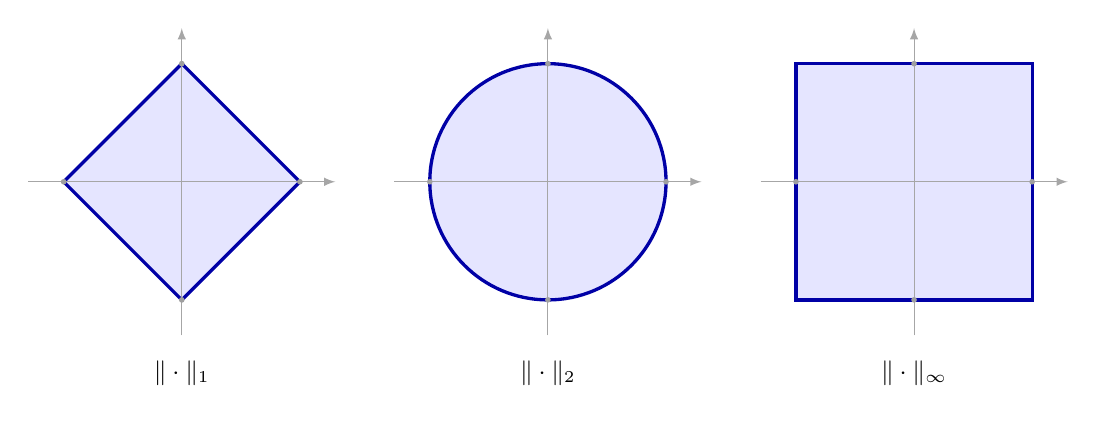
\begin{tikzpicture}[scale=1.5,>=latex]
  % rellenos primero
  \draw[very thick,blue!65!black,fill=blue!10] (1,0)--(0,1)--(-1,0)--(0,-1)--cycle;
  \begin{scope}[xshift=3.1cm]
    \draw[very thick,blue!65!black,fill=blue!10] (0,0) circle (1);
  \end{scope}
  \begin{scope}[xshift=6.2cm]
    \draw[very thick,blue!65!black,fill=blue!10] (-1,-1) rectangle (1,1);
  \end{scope}
  % ejes por encima
  \foreach \dx/\nombre in {0/{$\|\cdot\|_1$}, 3.1/{$\|\cdot\|_2$}, 6.2/{$\|\cdot\|_\infty$}}{
    \begin{scope}[xshift=\dx cm]
      \draw[->,gray!70] (-1.3,0) -- (1.3,0);
      \draw[->,gray!70] (0,-1.3) -- (0,1.3);
      \foreach \p in {(1,0),(0,1),(-1,0),(0,-1)}{\fill[gray!75] \p circle (0.024);}
      \node[font=\small] at (0,-1.62) {\nombre};
    \end{scope}
  }
\end{tikzpicture}
\caption{Las bolas unitarias de $\|\cdot\|_1$, $\|\cdot\|_2$ y
$\|\cdot\|_\infty$ en $\R^2$. Están encajadas,
$B_1\subseteq B_2\subseteq B_\infty$, y esas inclusiones son exactamente las
desigualdades $\|\bx\|_\infty\le\|\bx\|_2\le\|\bx\|_1$: cuanto más chica la
bola, más grande la norma.}
\label{fig:bolas}
\end{figure}

Las tres bolas son convexas y simétricas respecto del origen; eso no es
casualidad --- lo garantizan (n3) y (n1) --- y de hecho toda región convexa,
simétrica y acotada con el origen en su interior es la bola unitaria de
alguna norma. Las diferencias entre ellas están en las esquinas, y son las
que importan en la práctica: la bola de $\ell^1$ tiene vértices sobre los
ejes coordenados, es decir en vectores con coordenadas nulas.

\begin{remark}[Por qué $\ell^1$ produce soluciones ralas]
\label{obs:ralas}
Supongamos que buscamos, entre todos los $\bv$ de una recta dada del plano,
el de norma mínima. Geométricamente: inflamos la bola unitaria hasta que
toque la recta. Con $\|\cdot\|_2$ el contacto ocurre en un punto cualquiera,
donde el disco es suave. Con $\|\cdot\|_1$ el contacto ocurre casi siempre en
un \emph{vértice} del rombo, o sea en un vector con una coordenada igual a
cero. Esa observación --- que se generaliza a $\R^n$, donde los vértices de
$B_1$ tienen $n-1$ coordenadas nulas --- es la razón de fondo por la que
penalizar con $\|\cdot\|_1$ en un problema de ajuste (el método conocido como
\emph{lasso}) selecciona automáticamente unas pocas variables, mientras que
penalizar con $\|\cdot\|_2$ (\emph{ridge}) achica todos los coeficientes sin
anular ninguno. Es la Entrega~\ref{ent:bolas}.
\end{remark}

\subsection{Normas equivalentes}

Las desigualdades que se leen en la Figura~\ref{fig:bolas} se pueden dar
vuelta y acotar en los dos sentidos: en $\R^n$ vale
\[
\|\bx\|_\infty\le\|\bx\|_2\le\sqrt n\,\|\bx\|_\infty,
\qquad
\|\bx\|_2\le\|\bx\|_1\le\sqrt n\,\|\bx\|_2 .
\]
Dos normas $\|\cdot\|_a$ y $\|\cdot\|_b$ sobre un mismo espacio se dicen
\textbf{equivalentes} si existen constantes $0<c\le C$ con
\[
c\,\|\bx\|_a\le\|\bx\|_b\le C\,\|\bx\|_a \qquad\text{para todo }\bx .
\]
Vale el siguiente teorema, que no demostraremos porque requiere argumentos de
compacidad que exceden estas notas.

\begin{theorem}\label{teo:equivalencia}
En un espacio vectorial de dimensión finita, todas las normas son
equivalentes.
\end{theorem}

La consecuencia práctica es grande: en $\R^n$, una sucesión converge en una
norma si y sólo si converge en cualquier otra, y al mismo límite. Uno puede
entonces elegir la norma que le resulte más cómoda para estimar, sin cambiar
qué converge y qué no. (En dimensión infinita el teorema es falso, y ahí la
elección de la norma sí cambia el problema.)

\begin{entrega}{Bolas unitarias y soluciones ralas}\label{ent:bolas}
Trabajamos en $\R^2$ salvo aviso.
\begin{enumerate}[label=\textbf{(\alph*)},itemsep=3pt,topsep=4pt]
\item Dibujar con cuidado $B_1$, $B_2$ y $B_\infty$ en un mismo gráfico.
Probar las inclusiones $B_1\subseteq B_2\subseteq B_\infty$ y escribir las
desigualdades entre normas equivalentes a ellas.

\item Probar que en $\R^n$ valen
$\|\bx\|_\infty\le\|\bx\|_2\le\sqrt n\,\|\bx\|_\infty$ y
$\|\bx\|_2\le\|\bx\|_1\le\sqrt n\,\|\bx\|_2$, indicando en cada una para qué
vectores hay igualdad. \emph{Sugerencia:} para la última, aplicar
Cauchy-Schwarz a $\bx$ y al vector de signos de sus coordenadas.

\item Sea $L=\{\bv\in\R^2 : a_1v_1+a_2v_2=1\}$ una recta que no pasa por el
origen, con $a_1,a_2>0$ distintos. Calcular el mínimo de $\|\bv\|_2$ sobre
$L$ y el punto donde se alcanza. Repetir con $\|\bv\|_1$ y con
$\|\bv\|_\infty$.

\item Interpretar el ítem (c) geométricamente: el mínimo se alcanza donde la
bola $\{\|\bv\|\le t\}$, al inflarse, toca $L$ por primera vez. Explicar por
qué con $\|\cdot\|_1$ el contacto ocurre en un vértice del rombo --- salvo
para pendientes excepcionales que hay que identificar --- y por qué eso
significa que el minimizador tiene una coordenada nula.

\item Generalizar en palabras a $\R^n$: describir los vértices de $B_1$ y
decir cuántas coordenadas nulas tiene un vector que esté en uno de ellos.
Explicar en una o dos frases por qué penalizar con $\|\cdot\|_1$ selecciona
variables (\emph{lasso}) y penalizar con $\|\cdot\|_2$ no (\emph{ridge}).

\item Verificar que $\|\bx\|_p$ \emph{no} es una norma para $0<p<1$, usando
$\bx=(1,0)$ e $\by=(0,1)$. ¿Qué le pasa a la ``bola unitaria'' en ese caso?
\end{enumerate}

\medskip
\noindent{\footnotesize\emph{Se entrega por escrito. Los ítems (d) y (e) son
la explicación geométrica estándar de por qué la regularización $\ell^1$
produce modelos ralos.}}
\end{entrega}

% ===================================================================
\subsection{Normas de matrices}

Como $\R^{m\times n}$ es un espacio vectorial de dimensión $mn$, todo lo
anterior se aplica a matrices sin cambiar una coma: alcanza con leer una
matriz como un vector largo. Así se obtiene la \textbf{norma de Frobenius}
que ya definimos en la Sección~\ref{sec:frobenius},
\[
\|A\|_F=\sqrt{\sum_{i=1}^{m}\sum_{j=1}^{n}a_{ij}^2}=\sqrt{\tr(A^TA)},
\]
que no es otra cosa que la norma $\|\cdot\|_2$ de $\R^{mn}$.

Hay otra manera de medir una matriz, que no viene de olvidarse de que es una
matriz sino justamente de usarlo: mirar cuánto estira. Es la \textbf{norma
espectral}
\[
\|A\|_2=\max_{\|\bx\|_2=1}\|A\bx\|_2
=\max_{\bx\neq0}\frac{\|A\bx\|_2}{\|\bx\|_2} .
\]
Acá hay algo que podría pasar desapercibido: \emph{ese máximo ya sabemos que
existe}. No hace falta esperar a ningún capítulo posterior. En efecto, si
$\|\bx\|_2=1$,
\[
\|A\bx\|_2^2=(A\bx)^T(A\bx)=\bx^T(A^TA)\bx ,
\]
y $A^TA$ es simétrica y semidefinida positiva, de modo que el
Teorema~\ref{teo:rayleigh} del Capítulo~\ref{cap:sdp} dice que el máximo de
esa energía sobre la esfera unitaria es $\lambda_1(A^TA)$, alcanzado en el
autovector correspondiente. Es decir,
\begin{equation}\label{eq:espectral-rayleigh}
\|A\|_2=\sqrt{\lambda_1(A^TA)} .
\end{equation}
Lo que falta no es la existencia sino el \emph{nombre} y la factorización que
lo acompaña: a ese número se lo llama el mayor \emph{valor singular} de $A$ y
se lo escribe $\sigma_1$, y de ahí en adelante empieza el
Capítulo~\ref{cap:SVD}. La familia general de normas definidas por un máximo
como éste ---una por cada norma vectorial--- es el tema del
Capítulo~\ref{cap:normas-matrices}.

El caso simétrico sale del mismo teorema y conviene hacerlo acá, porque hay
una trampa.

\begin{proposition}\label{prop:normaS-espectral}
Si $S\in\R^{n\times n}$ es simétrica con autovalores
$\lambda_1,\dots,\lambda_n$, entonces
\[
\|S\|_2=\max_{i}|\lambda_i| .
\]
\end{proposition}

\begin{proof}
Por~\eqref{eq:espectral-rayleigh} con $A=S$, es
$\|S\|_2^2=\lambda_1(S^TS)=\lambda_1(S^2)$. Ahora bien, si $S=Q\Lambda Q^T$
es el teorema espectral, entonces $S^2=Q\Lambda^2Q^T$: los autovalores de
$S^2$ son los $\lambda_i^2$, con los mismos autovectores. El mayor de ellos
es $\max_i\lambda_i^2$, y tomando raíz cuadrada queda $\max_i|\lambda_i|$.
\end{proof}

\begin{remark}[Dos máximos que no son el mismo]\label{obs:dos-maximos}
Para una matriz simétrica conviven dos cantidades que es fácil confundir:
\[
\max_{\|\bx\|_2=1}\ \bx^TS\bx=\lambda_1
\qquad\text{y}\qquad
\max_{\|\bx\|_2=1}\ \|S\bx\|_2=\max_i|\lambda_i| .
\]
La primera es el máximo de la \emph{energía} y lleva el signo; la segunda es
el máximo \emph{estiramiento} y mira el módulo. Coinciden si $S$ es
semidefinida positiva ---ahí todos los autovalores son $\ge0$--- y en
general no: para $S=\diag(1,-5)$ la energía máxima es $1$ y la norma
espectral es $5$. La primera es el Teorema~\ref{teo:rayleigh} tal cual; la
segunda es ese teorema aplicado a $S^2$, que es donde desaparecen los signos.
\end{remark}

\subsection{¿Toda distancia viene de una norma?}

No. Ya vimos que una distancia puede vivir en un conjunto que ni siquiera es
un espacio vectorial, y aun sobre un espacio vectorial la distancia
discreta~\eqref{eq:discreta} no puede provenir de ninguna norma: si viniera
de $\|\cdot\|$, tendríamos $d(2\bx,\bi 0)=2\,d(\bx,\bi 0)$ para todo $\bx$,
imposible si $d$ sólo toma los valores $0$ y $1$. Las dos propiedades que
delatan a las que sí provienen de una norma son precisamente las que acabamos
de usar.

\begin{thm}\label{teo-normasdistancias}
Sea $\VV$ un espacio vectorial y $d$ una distancia en $\VV$. Entonces $d$ es
inducida por alguna norma si y sólo si para todos $\bx,\by\in\VV$ satisface
\begin{enumerate}[label=\textup{(\alph*)}]
\item $d(\bx+\ba,\by+\ba)=d(\bx,\by)$ para todo $\ba\in\VV$
\hfill (invarianza traslacional) \label{itm:trasl}
\item $d(\lambda\bx,\lambda\by)=|\lambda|\,d(\bx,\by)$ para todo
$\lambda\in\R$ \hfill (homogeneidad) \label{itm:hom}
\end{enumerate}
En ese caso la norma es $\|\bx\|=d(\bx,\bi 0)$.
\end{thm}

La prueba es el Ejercicio~\ref{ejer-teonormadistancia}.

% ===================================================================
\section{Productos internos}
\label{sec:productos-internos}

\begin{definition}
Sea $\VV$ un espacio vectorial sobre $\R$. Una función
$\langle\cdot,\cdot\rangle:\VV\times\VV\to\R$ es un \textbf{producto
interno} si para todo $\bx,\by,\bi{z}\in\VV$ y $c\in\R$:
\begin{enumerate}[label=\textup{(p\arabic*)}]
\item\label{item-pi-simetria} $\langle\bx,\by\rangle=\langle\by,\bx\rangle$
\item\label{item-pi-homo} $\langle c\bx,\by\rangle=c\langle\bx,\by\rangle$
\item\label{item-pi-adit} $\langle\bx+\by,\bi{z}\rangle
  =\langle\bx,\bi{z}\rangle+\langle\by,\bi{z}\rangle$
\item\label{item-pi-conf} $\langle\bx,\bx\rangle\ge0$, y
  $\langle\bx,\bx\rangle=0$ si y sólo si $\bx=0$
\end{enumerate}
\end{definition}

Los ítems \ref{item-pi-homo} y \ref{item-pi-adit} dicen que
$\langle\cdot,\cdot\rangle$ es lineal en la primera variable; por
\ref{item-pi-simetria} también lo es en la segunda. Es decir: una forma
bilineal, simétrica y definida positiva.

\begin{example}\label{ej:productos-internos}
Tres ejemplos que ya conocemos, cada uno en su espacio:
\begin{enumerate}[label=\textup{(\arabic*)},itemsep=2pt]
\item El \textbf{producto escalar usual} en $\R^n$,
$\langle\bx,\by\rangle=\bx^T\by=\sum_i x_iy_i$, que es el del
Capítulo~\ref{cap:ortogonalidad}.
\item El \textbf{producto asociado a una matriz sdp}: si $S\in\R^{n\times n}$
es sdp, $\langle\bx,\by\rangle_S=\bx^TS\by$ es un producto interno en $\R^n$
(Entrega~\ref{ent:elipses}, ítem (d)). Con $S=I$ se recupera el anterior.
\item El \textbf{producto de Frobenius} en $\R^{m\times n}$,
$\langle A,B\rangle_F=\tr(A^TB)$, de la Sección~\ref{sec:frobenius}.
\end{enumerate}
\end{example}

Todo producto interno trae consigo una longitud:
\begin{equation}\label{eq-normaPI}
\|\bx\|=\sqrt{\langle\bx,\bx\rangle} .
\end{equation}
Que esto sea efectivamente una norma lo probaremos enseguida. Lo importante
es lo que viene primero.

\subsection{\texorpdfstring{Todo el Capítulo~\ref{cap:ortogonalidad}, otra vez}{Todo el capitulo de ortogonalidad, otra vez}}

En el Capítulo~\ref{cap:ortogonalidad} probamos, para $\R^n$ con el producto
usual, la desigualdad de Cauchy-Schwarz (Teorema~\ref{teo:cauchy-schwarz}),
la desigualdad triangular, el teorema de Pitágoras
(Teorema~\ref{teo:pitagoras}) y la definición del ángulo por
$\cos\theta=\bx^T\by/(\|\bx\|\|\by\|)$. Vale la pena releer aquellas
demostraciones con esta pregunta en la cabeza: \emph{¿en qué lugar se usó que
el espacio era $\R^n$, o que el producto era $\sum_ix_iy_i$?}

La respuesta es: en ninguno. Todas las cuentas fueron desarrollar cuadrados,
sacar escalares afuera y usar que $\|\bi{v}\|^2\ge0$ --- es decir,
exactamente \ref{item-pi-simetria}--\ref{item-pi-conf}. Por lo tanto:

\begin{theorem}[Cauchy-Schwarz]\label{teo-cs}
Sea $\VV$ un espacio vectorial con producto interno y $\|\cdot\|$ la norma
\eqref{eq-normaPI}. Entonces, para todos $\bx,\by\in\VV$,
\[
|\langle\bx,\by\rangle|\le\|\bx\|\,\|\by\| ,
\]
con igualdad si y sólo si $\bx$ e $\by$ son linealmente dependientes.
\end{theorem}

\begin{proof}
Es, palabra por palabra, la demostración del
Teorema~\ref{teo:cauchy-schwarz}: si $\bx=0$ no hay nada que probar, y si no,
el polinomio
\[
p(t)=\|t\bx+\by\|^2=t^2\|\bx\|^2+2t\,\langle\bx,\by\rangle+\|\by\|^2
\]
es no negativo para todo $t$, luego su discriminante
$4\langle\bx,\by\rangle^2-4\|\bx\|^2\|\by\|^2$ es $\le0$. Hay igualdad
exactamente cuando $p$ tiene una raíz doble $t_0$, es decir cuando
$\by=-t_0\bx$.
\end{proof}

\begin{theorem}[Pitágoras]\label{teo-pitagoras-gral}
Si $\langle\bx,\by\rangle=0$, entonces
$\|\bx\pm\by\|^2=\|\bx\|^2+\|\by\|^2$.
\end{theorem}

\begin{proof}
La del Teorema~\ref{teo:pitagoras}: desarrollar
$\|\bx\pm\by\|^2=\langle\bx\pm\by,\bx\pm\by\rangle
=\|\bx\|^2\pm2\langle\bx,\by\rangle+\|\by\|^2$ y anular el término del medio.
\end{proof}

Con Cauchy-Schwarz podemos definir el \textbf{ángulo} entre dos vectores no
nulos de $\VV$ por
\begin{equation}\label{eq:angulo-general}
\cos\theta=\frac{\langle\bx,\by\rangle}{\|\bx\|\,\|\by\|}\in[-1,1] ,
\end{equation}
y decimos que $\bx$ e $\by$ son \textbf{ortogonales}, $\bx\perp\by$, cuando
$\langle\bx,\by\rangle=0$. Insistimos en el punto, porque es el que usaremos
en todo lo que sigue: \emph{cambiar el producto interno cambia qué vectores
son ortogonales y cuánto mide el ángulo entre dos vectores dados.}

Recién ahora podemos cerrar la promesa pendiente.

\begin{theorem}\label{teo-normapi}
Si $\VV$ tiene un producto interno, entonces
$\|\bx\|=\sqrt{\langle\bx,\bx\rangle}$ es una norma en $\VV$.
\end{theorem}

\begin{proof}
(n2) es exactamente \ref{item-pi-conf}. Para (n1),
\[
\|c\bx\|=\sqrt{\langle c\bx,c\bx\rangle}=\sqrt{c^2\langle\bx,\bx\rangle}
=|c|\,\|\bx\| ,
\]
usando \ref{item-pi-homo} en las dos variables. Para (n3), desarrollamos el
cuadrado y acotamos el término cruzado con Cauchy-Schwarz:
\[
\|\bx+\by\|^2=\|\bx\|^2+2\langle\bx,\by\rangle+\|\by\|^2
\le\|\bx\|^2+2\|\bx\|\,\|\by\|+\|\by\|^2=(\|\bx\|+\|\by\|)^2 . \qedhere
\]
\end{proof}

\subsection{¿Toda norma viene de un producto interno?}

Tampoco. Y el criterio para decidirlo es una identidad puramente métrica.

\begin{prop}\label{propo-propPI}
Sea $\VV$ un espacio con producto interno y $\|\cdot\|$ la norma
\eqref{eq-normaPI}. Entonces, para $\bx,\by\in\VV$,
\begin{enumerate}[label=\textup{(\alph*)},itemsep=2pt]
\item \textup{\textbf{Ley del paralelogramo:}}
$\|\bx+\by\|^2+\|\bx-\by\|^2=2\big(\|\bx\|^2+\|\by\|^2\big)$.
\item \textup{\textbf{Identidad de polarización:}}
$\displaystyle\langle\bx,\by\rangle
=\tfrac14\big(\|\bx+\by\|^2-\|\bx-\by\|^2\big)$.
\end{enumerate}
\end{prop}

\begin{proof}
Desarrollando, $\|\bx\pm\by\|^2=\|\bx\|^2\pm2\langle\bx,\by\rangle+\|\by\|^2$.
Sumando las dos igualdades sale (a); restándolas, (b).
\end{proof}

Las dos dicen cosas distintas y conviene no confundirlas. La ley del
paralelogramo es una \emph{restricción} sobre la norma: relaciona las
diagonales de un paralelogramo con sus lados, y no toda norma la cumple. La
identidad de polarización es una \emph{fórmula de recuperación}: muestra que
el producto interno queda determinado por su norma, de modo que no puede
haber dos productos internos distintos con la misma norma.

\begin{example}\label{ej:infinito-no}
En $\R^2$ con $\|\cdot\|_\infty$, tomemos $\bx=(1,0)^T$ e $\by=(0,1)^T$.
Entonces $\bx+\by=(1,1)^T$ y $\bx-\by=(1,-1)^T$, de modo que
\[
\|\bx+\by\|_\infty^2+\|\bx-\by\|_\infty^2=1+1=2,
\qquad
2\big(\|\bx\|_\infty^2+\|\by\|_\infty^2\big)=2(1+1)=4 .
\]
La ley del paralelogramo falla, y por el teorema que sigue $\|\cdot\|_\infty$
no proviene de ningún producto interno. El mismo par de vectores sirve para
$\|\cdot\|_1$.
\end{example}

\begin{thm}[Jordan--von Neumann]\label{teo-normaPI-carac}
Sea $\VV$ un espacio vectorial y $\|\cdot\|$ una norma sobre $\VV$. Existe un
producto interno que induce $\|\cdot\|$ si y sólo si $\|\cdot\|$ satisface la
ley del paralelogramo.
\end{thm}

\begin{proof}
Si $\|\cdot\|$ viene de un producto interno, la ley vale por la
Proposición~\ref{propo-propPI}.

Supongamos ahora que la norma satisface la ley del paralelogramo. Definimos
el candidato a producto interno por la identidad de polarización:
\[
\langle\bx,\by\rangle=\tfrac14\big(\|\bx+\by\|^2-\|\bx-\by\|^2\big) .
\]

\emph{Simetría \ref{item-pi-simetria}.} Como $\|\bi{w}\|=\|-\bi{w}\|$, es
$\|\bx+\by\|=\|\by+\bx\|$ y $\|\bx-\by\|=\|\by-\bx\|$, de donde
$\langle\bx,\by\rangle=\langle\by,\bx\rangle$.

\emph{Aditividad \ref{item-pi-adit}.} Por la ley del paralelogramo aplicada a
$\bx+\bi{z}$ y $\by$,
\[
\|\bx+\by+\bi{z}\|^2=2\|\bx+\bi{z}\|^2+2\|\by\|^2-\|\bx-\by+\bi{z}\|^2 ,
\]
e intercambiando $\bx$ con $\by$,
\[
\|\bx+\by+\bi{z}\|^2=2\|\by+\bi{z}\|^2+2\|\bx\|^2-\|\by-\bx+\bi{z}\|^2 .
\]
Promediando ambas,
\[
\|\bx+\by+\bi{z}\|^2=\|\bx\|^2+\|\by\|^2+\|\bx+\bi{z}\|^2+\|\by+\bi{z}\|^2
-\tfrac12\|\bx-\by+\bi{z}\|^2-\tfrac12\|\by-\bx+\bi{z}\|^2 .
\]
Reemplazando $\bi{z}$ por $-\bi{z}$ y usando $\|\bi{w}\|=\|-\bi{w}\|$ en los
dos últimos términos, que quedan iguales,
\[
\|\bx+\by-\bi{z}\|^2=\|\bx\|^2+\|\by\|^2+\|\bx-\bi{z}\|^2+\|\by-\bi{z}\|^2
-\tfrac12\|\bx-\by-\bi{z}\|^2-\tfrac12\|\by-\bx-\bi{z}\|^2 .
\]
Restando las dos últimas igualdades y dividiendo por $4$,
\[
\langle\bx+\by,\bi{z}\rangle
=\tfrac14\big(\|\bx+\bi{z}\|^2-\|\bx-\bi{z}\|^2\big)
+\tfrac14\big(\|\by+\bi{z}\|^2-\|\by-\bi{z}\|^2\big)
=\langle\bx,\bi{z}\rangle+\langle\by,\bi{z}\rangle .
\]

\emph{Positividad \ref{item-pi-conf}.} Directamente,
\[
\langle\bx,\bx\rangle=\tfrac14\big(\|2\bx\|^2-\|\bi 0\|^2\big)
=\tfrac14\cdot 4\|\bx\|^2=\|\bx\|^2 ,
\]
que es $\ge0$ y se anula sólo si $\bx=0$. De paso, esto confirma que el
producto interno construido induce la norma de partida.

\emph{Homogeneidad \ref{item-pi-homo}.} Es la única parte laboriosa. De la
aditividad sale $\langle n\bx,\by\rangle=n\langle\bx,\by\rangle$ para
$n\in\mathbb{N}$ por inducción, de ahí para $n\in\mathbb{Z}$ (usando
$\langle-\bx,\by\rangle=-\langle\bx,\by\rangle$, que se ve directo en la
fórmula), y de ahí para todo racional $q=m/n$ escribiendo
$n\langle q\bx,\by\rangle=\langle m\bx,\by\rangle$. Para pasar a los reales
se usa que $c\mapsto\langle c\bx,\by\rangle$ es continua, por serlo la norma,
y que los racionales son densos. Los detalles son el
Ejercicio~\ref{ej-homoPI}.
\end{proof}

% ===================================================================
\section{Los productos internos de $\R^n$ son las matrices sdp}
\label{sec:pi-sdp}

Volvemos a $\R^n$, que es donde trabajamos. La pregunta natural es cuántos
productos internos hay. La respuesta es completa y es la bisagra de todo el
capítulo.

\begin{theorem}\label{teo:pi-son-sdp}
Sea $\langle\cdot,\cdot\rangle$ una función de $\R^n\times\R^n$ en $\R$.
Entonces $\langle\cdot,\cdot\rangle$ es un producto interno si y sólo si
existe una matriz $S\in\R^{n\times n}$ sdp tal que
\[
\langle\bx,\by\rangle=\bx^T S\,\by \qquad\text{para todos }\bx,\by\in\R^n .
\]
Además $S$ es única, y está dada por $s_{ij}=\langle e_i,e_j\rangle$.
\end{theorem}

\begin{proof}
($\Leftarrow$) Si $S$ es sdp, la simetría \ref{item-pi-simetria} vale porque
$\bx^TS\by$ es un número, luego igual a su traspuesta $\by^TS^T\bx=\by^TS\bx$;
los ítems \ref{item-pi-homo} y \ref{item-pi-adit} son la linealidad del
producto de matrices; y \ref{item-pi-conf} es exactamente la definición de
definida positiva.

($\Rightarrow$) Sea $\langle\cdot,\cdot\rangle$ un producto interno y
definamos $s_{ij}=\langle e_i,e_j\rangle$. La matriz $S=(s_{ij})$ es
simétrica por \ref{item-pi-simetria}. Escribiendo
$\bx=\sum_i x_ie_i$ e $\by=\sum_j y_je_j$ y usando la bilinealidad,
\[
\langle\bx,\by\rangle
=\sum_{i=1}^n\sum_{j=1}^n x_iy_j\,\langle e_i,e_j\rangle
=\sum_{i,j} x_i s_{ij} y_j
=\bx^TS\by .
\]
Finalmente, $\bx^TS\bx=\langle\bx,\bx\rangle>0$ para $\bx\neq0$ por
\ref{item-pi-conf}, de modo que $S$ es sdp. La unicidad es inmediata:
$s_{ij}=e_i^TSe_j$ está forzado.
\end{proof}

La matriz $S$ se llama la \textbf{matriz de Gram} del producto interno en la
base canónica. Escribiremos de ahora en más
\[
\langle\bx,\by\rangle_S=\bx^TS\by,
\qquad
\|\bx\|_S=\sqrt{\bx^TS\bx},
\]
como en la Sección~\ref{sec:elipses}. El caso $S=I$ es el producto usual.

\begin{remark}[Qué dice el teorema]
Elegir una geometría en $\R^n$ --- una manera de medir longitudes y ángulos
que venga de un producto interno --- es exactamente elegir una matriz sdp. No
hay más opciones y no hay menos. Y como en el Capítulo~\ref{cap:sdp} vimos
que la matriz sdp $S$ está retratada por su elipse $\bx^TS\bx=1$, tenemos
también el diccionario geométrico: \emph{la elipse de $S$ es la
circunferencia unitaria del producto interno $\langle\cdot,\cdot\rangle_S$.}
Todo lo que sigue es leer ese diccionario.
\end{remark}

\begin{remark}[La distancia de Mahalanobis]
El ejemplo canónico en estadística: si $\Sigma$ es la matriz de covarianza de
un vector aleatorio, entonces $\Sigma^{-1}$ es sdp y
\[
d_{\Sigma}(\bx,\by)=\|\bx-\by\|_{\Sigma^{-1}}
=\sqrt{(\bx-\by)^T\Sigma^{-1}(\bx-\by)}
\]
es la \emph{distancia de Mahalanobis}. Mide en unidades de desviación
estándar y en las direcciones propias de los datos: dos puntos separados en
una dirección de mucha varianza están, para esta distancia, más cerca que dos
puntos igualmente separados en una dirección de poca varianza. Es la
distancia euclídea aplicada después de blanquear los datos, que es lo mismo
que decir $\|\bv\|_{\Sigma^{-1}}=\|\Sigma^{-1/2}\bv\|_2$.
\end{remark}

% ===================================================================
\section{$S$-ortogonalidad}
\label{sec:S-ortogonalidad}

Fijemos de acá en adelante $S\in\R^{n\times n}$ sdp, con autovalores
$\lambda_1\ge\cdots\ge\lambda_n>0$ y base ortonormal de autovectores
$\bq_1,\dots,\bq_n$, y sea $S^{1/2}$ su raíz cuadrada
(Sección~\ref{sec:raiz}).

\begin{definition}
Dos vectores $\bx,\by\in\R^n$ son \textbf{$S$-ortogonales} (o
\emph{conjugados respecto de $S$}) si
\[
\langle\bx,\by\rangle_S=\bx^TS\by=0 ,
\]
y lo escribimos $\bx\perp_S\by$. Una base $\bv_1,\dots,\bv_n$ de $\R^n$ es
\textbf{$S$-ortonormal} si $\bv_i^TS\bv_j=\delta_{ij}$, es decir, si la
matriz $V=[\,\bv_1\ \cdots\ \bv_n\,]$ cumple $V^TSV=I$.
\end{definition}

La herramienta que traduce todo al caso conocido es la raíz cuadrada:
\begin{equation}\label{eq:traduccion-S}
\boxed{\ \langle\bx,\by\rangle_S=(S^{1/2}\bx)^T(S^{1/2}\by),
\qquad
\|\bx\|_S=\|S^{1/2}\bx\|_2 .\ }
\end{equation}
En palabras: \emph{la geometría de $S$ es la geometría euclídea vista a
través de $S^{1/2}$}. Dos vectores son $S$-ortogonales exactamente cuando sus
imágenes por $S^{1/2}$ son ortogonales en el sentido usual, y una base es
$S$-ortonormal exactamente cuando $S^{1/2}V$ es ortogonal, o sea
$V=S^{-1/2}Q$ con $Q$ ortogonal.

\subsection{Cómo se ve la $S$-ortogonalidad}

El dibujo correcto es la elipse. Recordemos de la
Sección~\ref{sec:elipses} que
\[
E_S=\{\bx : \bx^TS\bx=1\}=\{\bx : \|\bx\|_S=1\}
\]
es un elipsoide de ejes $\bq_i$ y semiejes $1/\sqrt{\lambda_i}$: la
circunferencia unitaria de esta geometría.

Ahora bien, ¿cómo se reconoce un par $S$-ortogonal \emph{mirando la elipse}?
La respuesta clásica: son los \textbf{diámetros conjugados}. Sea $\bx\in E_S$
y consideremos la recta tangente a $E_S$ en $\bx$. Derivando
$\bx^TS\bx=1$ se ve que el vector normal (euclídeo) a esa tangente es
$S\bx$; por lo tanto la tangente tiene dirección $\by$ si y sólo si
$\by^TS\bx=0$, es decir si y sólo si $\by\perp_S\bx$. En resumen:

\begin{quote}
\emph{$\by$ es $S$-ortogonal a $\bx$ si y sólo si $\by$ es paralelo a la
recta tangente a la elipse $E_S$ en el punto $\bx$.}
\end{quote}

Para $S=I$ la elipse es una circunferencia, la tangente es perpendicular al
radio, y recuperamos la ortogonalidad de siempre. Para $S\neq I$ la tangente
ya no es perpendicular al radio y por eso dos vectores $S$-ortogonales se
ven, al ojo euclídeo, oblicuos (Figura~\ref{fig:s-ortogonal}).

\begin{figure}[htbp]
\centering
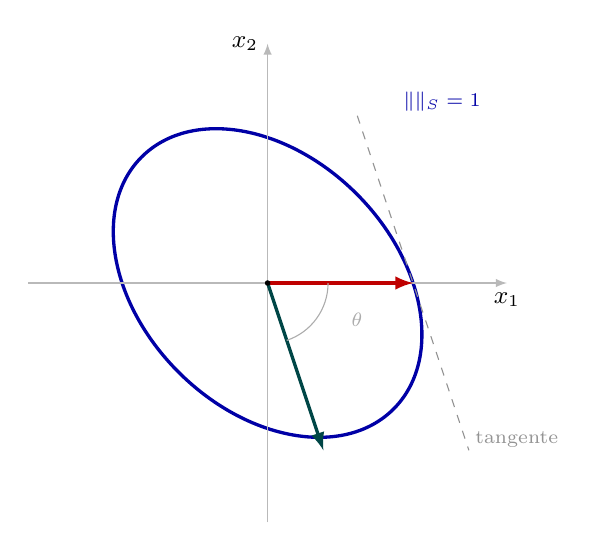
\begin{tikzpicture}[scale=3.2,>=latex]
  % --- elipse x^T S x = 1 para S=[[3,1],[1,3]] ---
  % semieje 1/2 en direccion (1,1) (lambda=4); semieje 1/sqrt2 en (1,-1) (lambda=2)
  \draw[very thick,blue!65!black,rotate=45] (0,0) ellipse (0.5 and 0.7071);
  \node[blue!65!black,font=\scriptsize,anchor=west] at (0.50,0.72) {$\|\bx\|_S=1$};
  % --- ejes coordenados, por encima del trazo ---
  \draw[->,gray!55] (-0.95,0) -- (0.95,0) node[below,black,font=\small] {$x_1$};
  \draw[->,gray!55] (0,-0.95) -- (0,0.95) node[left,black,font=\small] {$x_2$};
  % --- punto x = (1/sqrt3, 0) sobre la elipse, y la tangente alli ---
  \coordinate (X) at (0.5774,0);
  \draw[dashed,gray!85] (0.3560,0.6641) -- (0.7988,-0.6641);
  \node[gray!85,font=\scriptsize,anchor=west,inner sep=2pt] at (0.80,-0.62) {tangente};
  \draw[->,red!75!black,very thick] (0,0) -- (X);
  \node[red!75!black,font=\scriptsize,anchor=north,inner sep=3pt] at (0.50,-0.015) {$\bx$};
  % y S-ortogonal a x: misma direccion que la tangente
  \draw[->,teal!55!black,very thick] (0,0) -- (0.2214,-0.6641);
  \node[teal!55!black,font=\scriptsize,anchor=east,inner sep=3pt] at (0.175,-0.70) {$\by$};
  % angulo euclideo entre x e y
  \draw[gray!65] (0.24,0) arc (0:-71.6:0.24);
  \node[gray!65,font=\scriptsize] at (0.355,-0.145) {$\theta$};
  \fill (0,0) circle (0.011);
\end{tikzpicture}
\caption{$S$-ortogonalidad para $S=\left[\begin{smallmatrix}3&1\\1&3\end{smallmatrix}\right]$.
El vector $\by$ es $S$-ortogonal a $\bx$: es paralelo a la tangente a la
elipse en $\bx$. Al ojo euclídeo forman un ángulo $\theta\neq90^\circ$; en la
geometría de $S$ son perpendiculares. Si $S$ fuera $I$ la elipse sería una
circunferencia y la tangente, perpendicular al radio.}
\label{fig:s-ortogonal}
\end{figure}

\begin{remark}[Los autovectores no se enteran]
Los autovectores $\bq_i$ de $S$ son el único par de direcciones que es
ortogonal en los dos sentidos a la vez: si $i\neq j$,
\[
\bq_i^TS\bq_j=\lambda_j\,\bq_i^T\bq_j=0 .
\]
Son los ejes de la elipse, y una elipse es simétrica respecto de sus ejes. De
hecho $\bq_i/\sqrt{\lambda_i}$ es una base $S$-ortonormal: ya teníamos la
base, sólo hubo que reescalarla.
\end{remark}

\begin{entrega}{La geometría de una matriz sdp}\label{ent:geometria-S}
Sea $S\in\R^{n\times n}$ sdp con autovalores
$\lambda_1\ge\cdots\ge\lambda_n>0$ y autovectores ortonormales
$\bq_1,\dots,\bq_n$. Trabajamos con
$\langle\bx,\by\rangle_S=\bx^TS\by$ y $\|\bx\|_S=\sqrt{\bx^TS\bx}$.

\begin{enumerate}[label=\textbf{(\alph*)},itemsep=3pt,topsep=4pt]
\item Probar que $\langle\cdot,\cdot\rangle_S$ es un producto interno y que
$\|\cdot\|_S$ es una norma. \emph{Sugerencia:} lo segundo sale gratis del
Teorema~\ref{teo-normapi}, o bien de \eqref{eq:traduccion-S}; hacerlo de las
dos maneras.

\item En la Entrega~\ref{ent:elipses} del Capítulo~\ref{cap:sdp} probaron,
con el Teorema~\ref{teo:rayleigh}, que
$\sqrt{\lambda_n}\,\|\bx\|_2\le\|\bx\|_S\le\sqrt{\lambda_1}\,\|\bx\|_2$.
Releerlo con el vocabulario de este capítulo: deducir que $\|\cdot\|_S$ y
$\|\cdot\|_2$ son \emph{equivalentes} en el sentido de la
Sección~\ref{sec:bolas}, que las constantes son óptimas, y que la bola
$\{\|\bx\|_S\le1\}$ está encajada entre las bolas euclídeas de radios
$1/\sqrt{\lambda_1}$ y $1/\sqrt{\lambda_n}$. ¿Qué norma $\|\cdot\|_S$ da la
bola más parecida a la euclídea?

\item Probar que $\bx\perp_S\by$ si y sólo si
$S^{1/2}\bx\perp S^{1/2}\by$ en el sentido euclídeo. Deducir que
$\bv_1,\dots,\bv_n$ es una base $S$-ortonormal si y sólo si
$V=S^{-1/2}Q$ para alguna $Q$ ortogonal, y que por lo tanto hay infinitas.

\item \emph{(Diámetros conjugados.)} Sea $\bx$ con $\|\bx\|_S=1$. Probar que
el vector normal euclídeo a la elipse $E_S$ en el punto $\bx$ es $S\bx$, y
deducir que $\by\perp_S\bx$ si y sólo si $\by$ es paralelo a la tangente a
$E_S$ en $\bx$.

\item Tomar $S=\begin{bsmallmatrix}2&1\\ 1&2\end{bsmallmatrix}$. Dibujar
$E_S$; elegir $\bx=(1,0)^T/\sqrt2$ (verificar que está en $E_S$); encontrar
todos los $\by$ con $\bx\perp_S\by$; dibujarlos y comprobar sobre el dibujo
que son paralelos a la tangente. Calcular el ángulo euclídeo entre $\bx$ y
esos $\by$ y comprobar que no es recto.

\item Verificar que $\bq_i\perp_S\bq_j$ para $i\neq j$ y que
$\{\bq_i/\sqrt{\lambda_i}\}$ es base $S$-ortonormal. Explicar por qué los
autovectores son las únicas direcciones ortogonales en los dos sentidos a la
vez, usando el dibujo de la elipse.

\end{enumerate}

\medskip
\noindent{\footnotesize\emph{Se entrega por escrito. El ítem (c) es la clave
de todo: cambiar de producto interno es cambiar de coordenadas por
$S^{1/2}$. El (d) explica el dibujo de la Figura~\ref{fig:s-ortogonal}.}}
\end{entrega}

% ===================================================================
\subsection{Ángulos, Gram-Schmidt y proyecciones}

Todo lo que hicimos en el Capítulo~\ref{cap:ortogonalidad} se rehace
cambiando $\bx^T\by$ por $\bx^TS\by$, porque las demostraciones sólo usaban
los axiomas. En particular:

\begin{itemize}[itemsep=3pt]
\item El \textbf{ángulo $S$} entre $\bx$ e $\by$ no nulos es
$\cos\theta_S=\dfrac{\bx^TS\by}{\|\bx\|_S\|\by\|_S}$, y está en $[-1,1]$ por
Cauchy-Schwarz para $\langle\cdot,\cdot\rangle_S$.

\item \textbf{Gram-Schmidt} funciona igual: partiendo de una base cualquiera
$\ba_1,\dots,\ba_n$ y restando proyecciones $S$,
\[
\bv_k=\ba_k-\sum_{j<k}\frac{\langle \ba_k,\bv_j\rangle_S}{\langle \bv_j,\bv_j\rangle_S}\,\bv_j ,
\]
se obtiene una base $S$-ortogonal, y normalizando con $\|\cdot\|_S$, una
$S$-ortonormal. Todo subespacio tiene base $S$-ortonormal.

\item \textbf{Pitágoras} vale con $\perp_S$ y $\|\cdot\|_S$, y es lo que hace
que la proyección $S$ sea la mejor aproximación en $\|\cdot\|_S$.
\end{itemize}

Lo interesante es la proyección, porque ahí la diferencia con el caso
euclídeo se vuelve visible en la matriz. Sea $A\in\R^{n\times m}$ con
columnas linealmente independientes y sea $W=C(A)$. Queremos, dado $\bx$, el
punto de $W$ más cercano a $\bx$ \emph{en la métrica de $S$}; equivalentemente
(Pitágoras), el $P_S\bx\in W$ tal que el error $\bx-P_S\bx$ es
$S$-ortogonal a $W$.

Escribamos $P_S\bx=A\bi{c}$ e impongamos la condición. Que el error
$\bx-A\bi{c}$ sea $S$-ortogonal a todo $W=C(A)$ equivale a que lo sea a cada
elemento de una base de $W$, es decir, a cada columna
$\col_1(A),\dots,\col_m(A)$ de $A$:
\[
\left\{
\begin{aligned}
\col_1(A)^T S\,(\bx-A\bi{c}) &= 0 \\
&\ \,\vdots \\
\col_m(A)^T S\,(\bx-A\bi{c}) &= 0
\end{aligned}
\right.
\]
Ahora bien, $\col_j(A)^T$ es la fila $j$ de $A^T$, de modo que esas $m$
ecuaciones son las $m$ componentes de una sola ecuación matricial:
\[
A^T S\,(\bx-A\bi{c}) = \bi 0 .
\]
Distribuyendo llegamos a las \textbf{ecuaciones normales pesadas}
\begin{equation}\label{eq:normales-pesadas}
A^TSA\,\bi{c}=A^TS\bx .
\end{equation}
La matriz $A^TSA$ es sdp --- es el ítem (f) de la
Entrega~\ref{ent:minimos} --- luego invertible, y despejando:

\begin{equation}\label{eq:proyeccion-S}
\boxed{\ P_S=A\,(A^TSA)^{-1}A^TS\ }
\end{equation}

Con $S=I$ se recupera $P=A(A^TA)^{-1}A^T$ de
\eqref{eq:proyeccion-general}. La diferencia de fondo aparece al trasponer:

\begin{proposition}\label{prop:PS}
La matriz $P_S$ de \eqref{eq:proyeccion-S} cumple $P_S^2=P_S$ y $C(P_S)=C(A)$,
y es autoadjunta para $\langle\cdot,\cdot\rangle_S$, es decir
$\langle P_S\bx,\by\rangle_S=\langle\bx,P_S\by\rangle_S$ para todos
$\bx,\by$. Esto último equivale a que $SP_S$ sea simétrica. En general
$P_S\neq P_S^T$.
\end{proposition}

Es decir: \emph{$P_S$ es, en general, una proyección oblicua en el sentido
euclídeo}, de las que estudiamos en la Entrega~\ref{ent:oblicuas} --- $P^2=P$
pero $P\neq P^T$ ---, y sin embargo es una proyección \emph{ortogonal} para
la geometría de $S$. La misma matriz, dos lecturas. El criterio
``$P^2=P$ y $P=P^T$'' que caracterizaba a las proyecciones ortogonales se
transforma en

\begin{equation}\label{eq:criterio-PS}
P^2=P \quad\text{y}\quad SP=(SP)^T
\qquad\Longleftrightarrow\qquad
P \text{ es la proyección $S$-ortogonal sobre } C(P),
\end{equation}
que con $S=I$ es el criterio de siempre. Todo esto se demuestra en la
Entrega~\ref{ent:proyeccion-S}.

\begin{example}\label{ej:PS-recta}
Proyectemos sobre la recta generada por $\ba=(1,1)^T$ en $\R^2$, con
$S=\diag(1,4)$. La fórmula \eqref{eq:proyeccion-S} con $A=\ba$ da
$\ba^TS\ba=1+4=5$, $\ba^TS=(1,4)$, y
\[
P_S=\frac{1}{5}\begin{bmatrix}1\\ 1\end{bmatrix}\begin{bmatrix}1&4\end{bmatrix}
=\frac15\begin{bmatrix}1&4\\ 1&4\end{bmatrix} .
\]
Se verifica $P_S^2=P_S$, pero $P_S\neq P_S^T$; en cambio
$SP_S=\frac15\begin{bsmallmatrix}1&4\\ 4&16\end{bsmallmatrix}$ sí es
simétrica. Para $\bx=(0,1)^T$ resulta $P_S\bx=\frac45(1,1)^T$, mientras que
la proyección euclídea sería $\frac12(1,1)^T$: el peso $4$ en la segunda
coordenada hace que el error en esa dirección sea más caro, y la proyección
se corre para reducirlo.
\end{example}

\begin{remark}[Dónde aparece esto]
Tres lugares, el mismo cálculo. En \textbf{cuadrados mínimos con pesos}, uno
minimiza $\sum_i w_i\,(\text{residuo}_i)^2$ en lugar de la suma sin pesos:
eso es $\|A\bi{c}-\bi{b}\|_S^2$ con $S=\diag(w_1,\dots,w_n)$, y la solución
son las ecuaciones~\eqref{eq:normales-pesadas}. Se usa cuando los datos
tienen precisiones distintas; el peso óptimo es la inversa de la varianza, y
ahí reaparece Mahalanobis. En los \textbf{métodos de elementos finitos}, $S$
es la matriz de rigidez y la solución aproximada es la proyección
$S$-ortogonal de la solución exacta sobre el espacio de dimensión finita
elegido. Y en el \textbf{método del gradiente conjugado} para resolver
$S\bx=\bi{b}$, las direcciones de búsqueda sucesivas se eligen
$S$-ortogonales entre sí --- de ahí el nombre ``conjugado'' ---, y cada paso
es exactamente una proyección $S$-ortogonal.
\end{remark}

\begin{entrega}{La proyección $S$-ortogonal}\label{ent:proyeccion-S}
Sea $S\in\R^{n\times n}$ sdp, $A\in\R^{n\times m}$ con columnas linealmente
independientes, y
\[
P_S=A(A^TSA)^{-1}A^TS .
\]

\begin{enumerate}[label=\textbf{(\alph*)},itemsep=3pt,topsep=4pt]
\item Probar que $A^TSA$ es sdp, y en particular invertible, de modo que
$P_S$ está bien definida. \emph{Sugerencia:} $\bi{c}^TA^TSA\bi{c}=\|A\bi{c}\|_S^2$.

\item Probar que $P_S^2=P_S$, que $C(P_S)=C(A)$ y que $P_S\bx=\bx$ para todo
$\bx\in C(A)$. Deducir $\rg(P_S)=\tr(P_S)=m$.

\item Probar que $P_S$ es autoadjunta para $\langle\cdot,\cdot\rangle_S$, es
decir $\langle P_S\bx,\by\rangle_S=\langle\bx,P_S\by\rangle_S$ para todos
$\bx,\by$, y que esto equivale a que $SP_S$ sea simétrica.

\item Probar que el error es $S$-ortogonal al subespacio, en la forma
matricial $A^TS\,(\bx-P_S\bx)=\bi 0$, y explicar por qué esa única igualdad
dice exactamente que el error es $S$-ortogonal a cada columna de $A$ y, por
lo tanto, a todo $C(A)$. Deducir la
versión $S$ del teorema de la mejor aproximación,
\[
\|\bx-P_S\bx\|_S\le\|\bx-\bv\|_S \qquad\text{para todo }\bv\in C(A),
\]
con igualdad sólo si $\bv=P_S\bx$. \emph{Sugerencia:} Pitágoras con
$\perp_S$.

\item Probar que $P_S\bx=A\hat{\bi{c}}$ donde $\hat{\bi{c}}$ resuelve las
ecuaciones normales pesadas $A^TSA\,\hat{\bi{c}}=A^TS\bx$, y que $P_S$ no
depende de la base: si $B=AM$ con $M$ invertible, entonces
$B(B^TSB)^{-1}B^TS=P_S$.

\item \emph{(Recíproco.)} Probar que si $P\in\R^{n\times n}$ cumple $P^2=P$ y
$SP$ simétrica, entonces $P$ es la proyección $S$-ortogonal sobre $C(P)$.

\item \emph{(La conexión con las proyecciones oblicuas.)} Probar que
$P_S=S^{-1/2}\,\widetilde P\,S^{1/2}$, donde $\widetilde P$ es la proyección
ortogonal euclídea sobre $C(S^{1/2}A)$. Deducir que los autovalores de $P_S$
son $0$ y $1$, y que $\|P_S\bx\|_S\le\|\bx\|_S$ para todo $\bx$ --- aunque,
como se vio en la Entrega~\ref{ent:oblicuas}, el cociente
$\|P_S\bx\|_2/\|\bx\|_2$ pueda ser tan grande como se quiera. ¿Contradicción?
Explicar.

\item \emph{(Casos concretos.)}
\begin{enumerate}[label=\textup{(\roman*)},itemsep=2pt,topsep=3pt]
\item Con $\ba=(1,1,1)^T$ (una sola columna) y $S=\diag(1,2,3)$, calcular
$P_S$ y describir en palabras qué hace $P_S\bx$.
\item Con
$A=\begin{bsmallmatrix}1&0\\ 1&1\\ 0&1\end{bsmallmatrix}$ y
$S=\diag(1,2,1)$, calcular $P_S$, verificar $P_S^2=P_S$ y $\tr P_S=2$,
comprobar que $P_S\neq P_S^T$ pero que $SP_S$ sí es simétrica, y comparar con
la proyección usual ($S=I$).
\item \emph{(Una base $S$-ortonormal a mano.)} Aplicar Gram-Schmidt con
$\langle\cdot,\cdot\rangle_S$ a la base canónica de $\R^2$, con
$S=\begin{bsmallmatrix}2&1\\ 1&2\end{bsmallmatrix}$, y verificar que la base
obtenida cumple $V^TSV=I$. Dibujarla sobre la elipse $E_S$ y compararla con
la base $\{\bq_i/\sqrt{\lambda_i}\}$ de los autovectores reescalados.
\end{enumerate}
\end{enumerate}

\medskip
\noindent{\footnotesize\emph{Se entrega por escrito. El ítem (g) es el que
explica por qué una misma matriz puede ser ``oblicua'' y ``ortogonal'' al
mismo tiempo: depende de con qué producto interno se la mire. El (e) es el
punto de partida de los cuadrados mínimos con pesos.}}
\end{entrega}

% ===================================================================
\subsection{Resumen: el mismo capítulo dos veces}

\begin{center}
\renewcommand{\arraystretch}{1.35}
\begin{tabular}{@{}lll@{}}
\hline
 & \textbf{euclídeo} ($S=I$) & \textbf{geometría de $S$}\\
\hline
producto & $\bx^T\by$ & $\bx^TS\by$\\
norma & $\|\bx\|=\sqrt{\bx^T\bx}$ & $\|\bx\|_S=\sqrt{\bx^TS\bx}=\|S^{1/2}\bx\|$\\
esfera unitaria & circunferencia & elipse $\bx^TS\bx=1$\\
ortogonalidad & $\bx^T\by=0$ & $\bx^TS\by=0$ (diámetros conjugados)\\
base ortonormal & $Q^TQ=I$ & $V^TSV=I$, o sea $V=S^{-1/2}Q$\\
proyección sobre $C(A)$ & $A(A^TA)^{-1}A^T$ & $A(A^TSA)^{-1}A^TS$\\
criterio & $P^2=P$, $P=P^T$ & $P^2=P$, $SP$ simétrica\\
ecuaciones normales & $A^TA\bi{c}=A^T\bi{b}$ & $A^TSA\bi{c}=A^TS\bi{b}$\\
\hline
\end{tabular}
\end{center}

\medskip
La columna de la derecha no es una generalización gratuita: contiene a la
izquierda como el caso $S=I$, y todos sus enunciados se demuestran copiando
los de la izquierda, porque las pruebas nunca usaron más que los axiomas del
producto interno. Ése es, en definitiva, el argumento a favor de haber
definido las cosas abstractamente.


% ===================================================================
\section*{Ejercicios}

\begin{enumerate}

\item\label{ejer-normadistancia} Probar que en un espacio vectorial normado
$(\VV,\|\cdot\|)$ la función $d(\bx,\by)=\|\bx-\by\|$ es una distancia.

\item Probar que $\|\cdot\|_1$, $\|\cdot\|_2$ y $\|\cdot\|_\infty$ son normas
en $\R^n$. ¿Qué distancias inducen?

\item Probar que $\|A\|_F$ es una norma en $\R^{m\times n}$ de dos maneras:
directamente, y observando que proviene del producto interno de Frobenius.
Probar además que $\|A\|_F=\|A^T\|_F$ y que $\|QA\|_F=\|A\|_F$ si $Q$ es
ortogonal. \emph{Sugerencia:} $\|A\|_F^2=\tr(A^TA)$.

\item Mostrar directamente que para todo $\bi{v}\in\R^n$ vale
$\|\bi{v}\|_2^2\le\|\bi{v}\|_1\,\|\bi{v}\|_\infty$.

\item Mostrar que la distancia discreta es una distancia en cualquier
conjunto $\XX\neq\emptyset$. Si se la considera sobre un espacio vectorial
$\VV$, ¿puede existir alguna norma que la induzca?

\item\label{ejer-teonormadistancia} Demostrar el
Teorema~\ref{teo-normasdistancias}.

\item \textit{(Distancia del tren en Francia.)} Considerar en $\R^n$ la
función
\[
d(\bx,\by)=\begin{cases}
  d_2(\bx,\by) & \text{si }\bx=\alpha\by\text{ para algún }\alpha\in\R,\\
  d_2(\bx,\bi 0)+d_2(\bi 0,\by)& \text{en otro caso}.
\end{cases}
\]
Mostrar que es una distancia. ¿Puede ser inducida por alguna norma en $\R^2$?

\item\label{ejer-polarizacion} Demostrar la
Proposición~\ref{propo-propPI}, y verificar la ley del paralelogramo
explícitamente sobre $\R^2$ con $\|\cdot\|_2$ y sobre $\R^{2\times2}$ con
$\|\cdot\|_F$.

\item Sean $\VV$ un espacio vectorial con producto interno y $\|\cdot\|$ la
norma inducida. Probar que
\[
\|\bx\|=\sup_{\|\by\|=1}|\langle\bx,\by\rangle| ,
\]
e indicar dónde se alcanza el supremo.

\item\label{ejer-normainfty} Mostrar que $\|\cdot\|_1$ y $\|\cdot\|_\infty$
no provienen de ningún producto interno en $\R^n$, $n\ge2$.
\emph{Sugerencia:} Ejemplo~\ref{ej:infinito-no}.

\item\label{ejer-normaS} Dar una demostración de la
Proposición~\ref{prop:normaS-espectral} que no pase por $S^2$: escribir
$\bx$ en la base de autovectores de $S$, calcular $\|S\bx\|_2^2$
directamente y acotar como en el Teorema~\ref{teo:rayleigh}. Decir en qué
vectores se alcanza el máximo cuando hay dos autovalores de módulo máximo y
signos opuestos. ¿Qué parte del argumento se rompe si $S$ no es simétrica?

\item Probar que para toda $A\in\R^{m\times n}$ vale
$\|A\|_2\le\|A\|_F\le\sqrt{\rg(A)}\,\|A\|_2$. \emph{Sugerencia:} para la
primera, $\|A\bx\|_2\le\|A\|_F\|\bx\|_2$; la segunda es más fácil después del
Capítulo~\ref{cap:SVD}.

\item Probar que en un espacio con producto interno la convergencia
$\bx_k\to\bx$ (es decir $\|\bx_k-\bx\|\to0$) implica
$\langle\bx_k,\by\rangle\to\langle\bx,\by\rangle$ para todo $\by$ fijo.
\emph{Sugerencia:} Cauchy-Schwarz.

\item\label{ej-homoPI} \emph{(Homogeneidad en el Teorema~\ref{teo-normaPI-carac}.)}
En las condiciones de ese teorema, con
$\langle\bx,\by\rangle=\frac14(\|\bx+\by\|^2-\|\bx-\by\|^2)$, probar
sucesivamente:
\begin{enumerate}[label=\textup{(\alph*)}]
\item $\langle k\bx,\by\rangle=k\langle\bx,\by\rangle$ para $k\in\mathbb{N}$;
\item lo mismo para $k\in\mathbb{Z}$;
\item lo mismo para $k\in\mathbb{Q}$;
\item lo mismo para $k\in\R$, usando que $c\mapsto\langle c\bx,\by\rangle$ es
continua.
\end{enumerate}

\item\label{ejer-holder} Decimos que $p,q>1$ son \emph{exponentes conjugados}
si $\frac1p+\frac1q=1$. Demostraremos paso a paso la
\textbf{desigualdad de Hölder}: para todos
$\bx,\by\in\R^n$,
\[
\sum_{i=1}^n|x_iy_i|\le\Big(\sum_{i=1}^n|x_i|^p\Big)^{1/p}
\Big(\sum_{i=1}^n|y_i|^q\Big)^{1/q} .
\]
\begin{enumerate}
\item \textbf{Desigualdad de Young.} Demostrar que para $a,b\ge0$ y $p,q>1$
conjugados vale $ab\le\frac{a^p}{p}+\frac{b^q}{q}$.
\emph{Sugerencia:} estudiar $\varphi(t)=\frac{t^p}{p}+\frac1q-t$ para
$t\ge0$.

\item \textbf{Caso normalizado.} Sean
$A=\big(\sum_i|x_i|^p\big)^{1/p}$ y $B=\big(\sum_i|y_i|^q\big)^{1/q}$.
Mostrar que si $A=0$ o $B=0$ la desigualdad es trivial. En caso contrario,
definir $u_i=|x_i|/A$ y $v_i=|y_i|/B$ y verificar que
$\sum_iu_i^p=\sum_iv_i^q=1$.

\item \textbf{Aplicación de Young.} Aplicar el ítem 1 con $a=u_i$, $b=v_i$,
sumar en $i$ y usar las normalizaciones del ítem 2.

\item \textbf{Conclusión.} Escribir $u_iv_i=|x_i||y_i|/(AB)$ y deducir
Hölder. Observar que $p=q=2$ es Cauchy-Schwarz.

\item \textbf{Caso extremo.} Demostrar Hölder para $p=1$, $q=\infty$, donde
$\|\by\|_\infty=\max_i|y_i|$.

\item \textbf{Minkowski.} Deducir de Hölder que
$\|\bx+\by\|_p\le\|\bx\|_p+\|\by\|_p$, es decir, que $\|\cdot\|_p$ es una
norma. \emph{Sugerencia:} escribir
$\sum_i|x_i+y_i|^p\le\sum_i|x_i|\,|x_i+y_i|^{p-1}
+\sum_i|y_i|\,|x_i+y_i|^{p-1}$ y aplicar Hölder a cada sumando.
\end{enumerate}

\item Sea $S$ sdp y $\|\bx\|_S=\sqrt{\bx^TS\bx}$. Probar que $\|\cdot\|_S$
satisface la ley del paralelogramo, como debe ser por el
Teorema~\ref{teo-normaPI-carac}, y recuperar $\langle\cdot,\cdot\rangle_S$ a
partir de $\|\cdot\|_S$ por polarización.

\item Sea $S$ sdp. Probar que una matriz $U$ cumple $U^TSU=S$ si y sólo si
$U$ preserva el producto interno $\langle\cdot,\cdot\rangle_S$. Verificar que
estas matrices forman un grupo, y que para $S=I$ son exactamente las
ortogonales. ¿Qué transformaciones del plano son, geométricamente, cuando
$S=\diag(1,4)$?

\end{enumerate}
%\cite{horn}
